\documentclass{article}

% Language setting
% Replace `english' with e.g. `spanish' to change the document language
\usepackage[english]{babel}

% Set page size and margins
% Replace `letterpaper' with `a4paper' for UK/EU standard size
\usepackage[letterpaper,top=2cm,bottom=2cm,left=3cm,right=3cm,marginparwidth=1.75cm]{geometry}

% Useful packages
\usepackage{amsmath}
\usepackage{graphicx}
\usepackage[colorlinks=true, allcolors=blue]{hyperref}
\usepackage[backend=biber, style=apa]{biblatex}

\addbibresource{references.bib}

\title{Investigating Quantum Behavior Under Gravitational Waves: A Novel Experiment Combining Moving Double Slits and LIGO
}
\author{Dawid Zalewski, ChatGpt}

\begin{document}
\maketitle

\begin{abstract}
We propose an experiment to explore the interaction between gravitational waves and quantum particles by integrating LIGO with a modified double slit experiment. By comparing interference patterns in static and moving slit setups, while simultaneously detecting gravitational waves, we aim to observe quantum behavior under varying conditions. This novel design could provide insights into the relationship between quantum mechanics and general relativity. The results may lead to a deeper understanding of the influence of gravitational waves on quantum phenomena.
\end{abstract}

\section{Introduction}
Quantum mechanics and general relativity are the two foundational pillars of modern physics. While quantum mechanics explains the behavior of particles at the smallest scales, general relativity describes gravity and the structure of spacetime. However, there is a fundamental disconnect between these theories. Understanding how gravitational waves influence quantum particles may provide insights into this gap.

This paper presents an innovative experimental design combining LIGO with a modified double slit experiment to investigate the interplay between gravitational waves and quantum particles. We hypothesize that varying distances and motions of the double slits will yield distinct interference patterns, revealing gravitational influences on quantum phenomena. These findings could potentially bridge the gap between quantum mechanics and general relativity.

\section{Literature Review}
The intersection of quantum mechanics and gravitational wave physics has become a vibrant field of study, with various experiments aiming to unravel the complexities of quantum gravity. The double-slit experiment, first conducted by Thomas Young in 1801, showcased the wave-particle duality of light, serving as a foundational pillar in quantum mechanics. Recent advancements in quantum theory have expanded our understanding of this phenomenon, particularly regarding quantum superposition and entanglement (\cite{nielsen2010}).

The detection of gravitational waves by the Laser Interferometer Gravitational-Wave Observatory (LIGO) in 2015 marked a significant milestone, leading to new inquiries about the interplay between gravitational waves and quantum systems (\cite{abbott2016}). However, a gap remains in correlating gravitational waves with quantum phenomena. Studies have indicated potential connections between quantum fluctuations and gravitational waves, indicating that gravitational effects may influence quantum systems (\cite{maldacena2013}).

Several experiments have been proposed to investigate the quantum effects of gravity. One such proposal involves Entanglement Witness techniques, which aim to determine whether gravity can induce entanglement between massive particles. These experiments test the fundamental principles of quantum mechanics in the presence of gravitational fields, potentially revealing how gravity interacts with quantum systems (\cite{rangamani2017}).

Another notable study, "Testing the Quantumness of Gravity without Entanglement," explores how quantum effects can be observed in gravitational contexts without relying on entanglement. This research suggests that even classical gravity could exhibit quantum characteristics under specific conditions, providing insights into how gravity might operate at the quantum level (\cite{oppenheim2021}).

The moving double-slit experiment is a novel extension of the classic setup that offers insights into how particles behave in dynamic environments. Previous research has shown that the motion of slits can alter interference patterns, indicating that the wave function of particles can be affected by external conditions (\cite{scully1999}). Integrating this with gravitational wave detection could enhance our understanding of quantum interactions under extreme conditions.

Moreover, both analog and digital data capture methods are employed in quantum experiments and gravitational wave detection. The reliability of these data is critical for validating experimental results. Research on the limitations of digital versus analog data collection indicates that while digital systems offer precision and ease of analysis, analog systems are often considered more robust in certain experimental setups due to their longstanding application in physics (\cite{klyshko1988}).

By synthesizing insights from these diverse domains, this study aims to explore how gravitational waves interact with quantum particles, bridging the gap between quantum mechanics and general relativity.

\section{Methodology}

\subsection{Overview}
This experiment aims to study the effects of gravitational waves on quantum phenomena using a modified double-slit experiment combined with LIGO. The idea is to observe changes in interference patterns as gravitational waves pass through the region. 

To enhance the traditional double-slit setup, we introduce motion into both the slit and the photodetector. This modification allows for observations of quantum effects in dynamic systems, where spacetime motion and gravitational waves are at play. These enhancements provide a practical testbed for exploring quantum gravity.

\subsection{Technical Setup}
The technical details are as follows:

1. \textbf{LIGO System}: LIGO's two 4-kilometer arms use laser beams to detect minuscule changes in distance caused by gravitational waves.

2. \textbf{Double-Slit Apparatus}: Three experimental setups will be appended to LIGO's arms, each 1 kilometer in length and positioned 500 meters away to minimize interference. These setups are as follows:

   - \textbf{Static Slit Setup}: A traditional double-slit experiment where electrons pass through fixed slits, serving as a control to compare interference patterns in static conditions.
   
   - \textbf{Constant Velocity Slit Setup}: Slits are mounted on a rail system, moving at a constant velocity between two positions. This motion tests the effects of constant speed on quantum interference patterns.
   
   - \textbf{Accelerating Slit Setup}: Similar to the constant velocity setup, but the slits accelerate and decelerate as they move. This setup examines how changes in speed affect interference patterns.
\newline

Given the finite speed of gravitational waves, the separation between LIGO’s detection facility and our experimental setup introduces a delay of picoseconds or femtoseconds, which is below the threshold of human perception but must still be accounted for to ensure the accuracy of data correlation. The implementation of atomic clocks synchronized with LIGO’s detection timestamps is crucial for aligning the detection of gravitational waves with the timing of observations at the slits. This level of synchronization is essential for validating the impact of gravitational waves on the experimental apparatus.

\subsection{Control Measures}
Several control measures are in place to ensure the accuracy and reliability of results:

1. \textbf{Sanity Checks}: The static slit setup serves as a baseline, ensuring any observed effects in the moving setups are genuine and not artifacts.
   
2. \textbf{Calibration}: Regular calibration of both analog and digital equipment will reduce measurement errors and ensure consistency.
   
3. \textbf{Data Redundancy}: Both analog and digital data will be collected. Discrepancies will be cross-checked, with priority given to analog data due to its reliability.
   
4. \textbf{Limitations of Moving Slits}: To minimize interference, moving slits will be designed to have minimal moments of static positioning as they change direction. Electromagnetic shielding and physical separation will reduce noise and environmental disturbances.

5. \textbf{Vacuum Environment}: The arms and slits may need to be encased in a vacuum to prevent disturbances from air molecules, which could interfere with measurements during motion.

6. \textbf{Precision Rail System}: The rails will be straight and frictionless to reduce noise. Given LIGO's sensitivity, similar precision is required in the double-slit setups to ensure accurate quantum measurements under gravitational influence.

\subsection{Data Collection}
Both analog and digital data will be captured to ensure comprehensive analysis:

1. \textbf{Analog Data}: Photomultiplier tubes will count photons hitting the detectors, providing raw particle detection data.

2. \textbf{Digital Data}: High-resolution cameras and data acquisition systems will capture and analyze wave functions and interference patterns in real time.

\subsection{Data Analysis}
Collected data will be analyzed through the following steps:

1. \textbf{Pattern Recognition}: Software tools will identify and quantify interference patterns from all setups.
   
2. \textbf{Statistical Comparison}: Statistical analysis will compare interference patterns between the static, constant velocity, and accelerating setups, focusing on their correlation with gravitational waves.
   
3. \textbf{Error Analysis}: A comprehensive error analysis will account for any discrepancies between analog and digital data, including noise, calibration issues, and environmental influences.

\section{Experimental Setup and Diagram Explanation}

\begin{figure}[h]
    \centering
    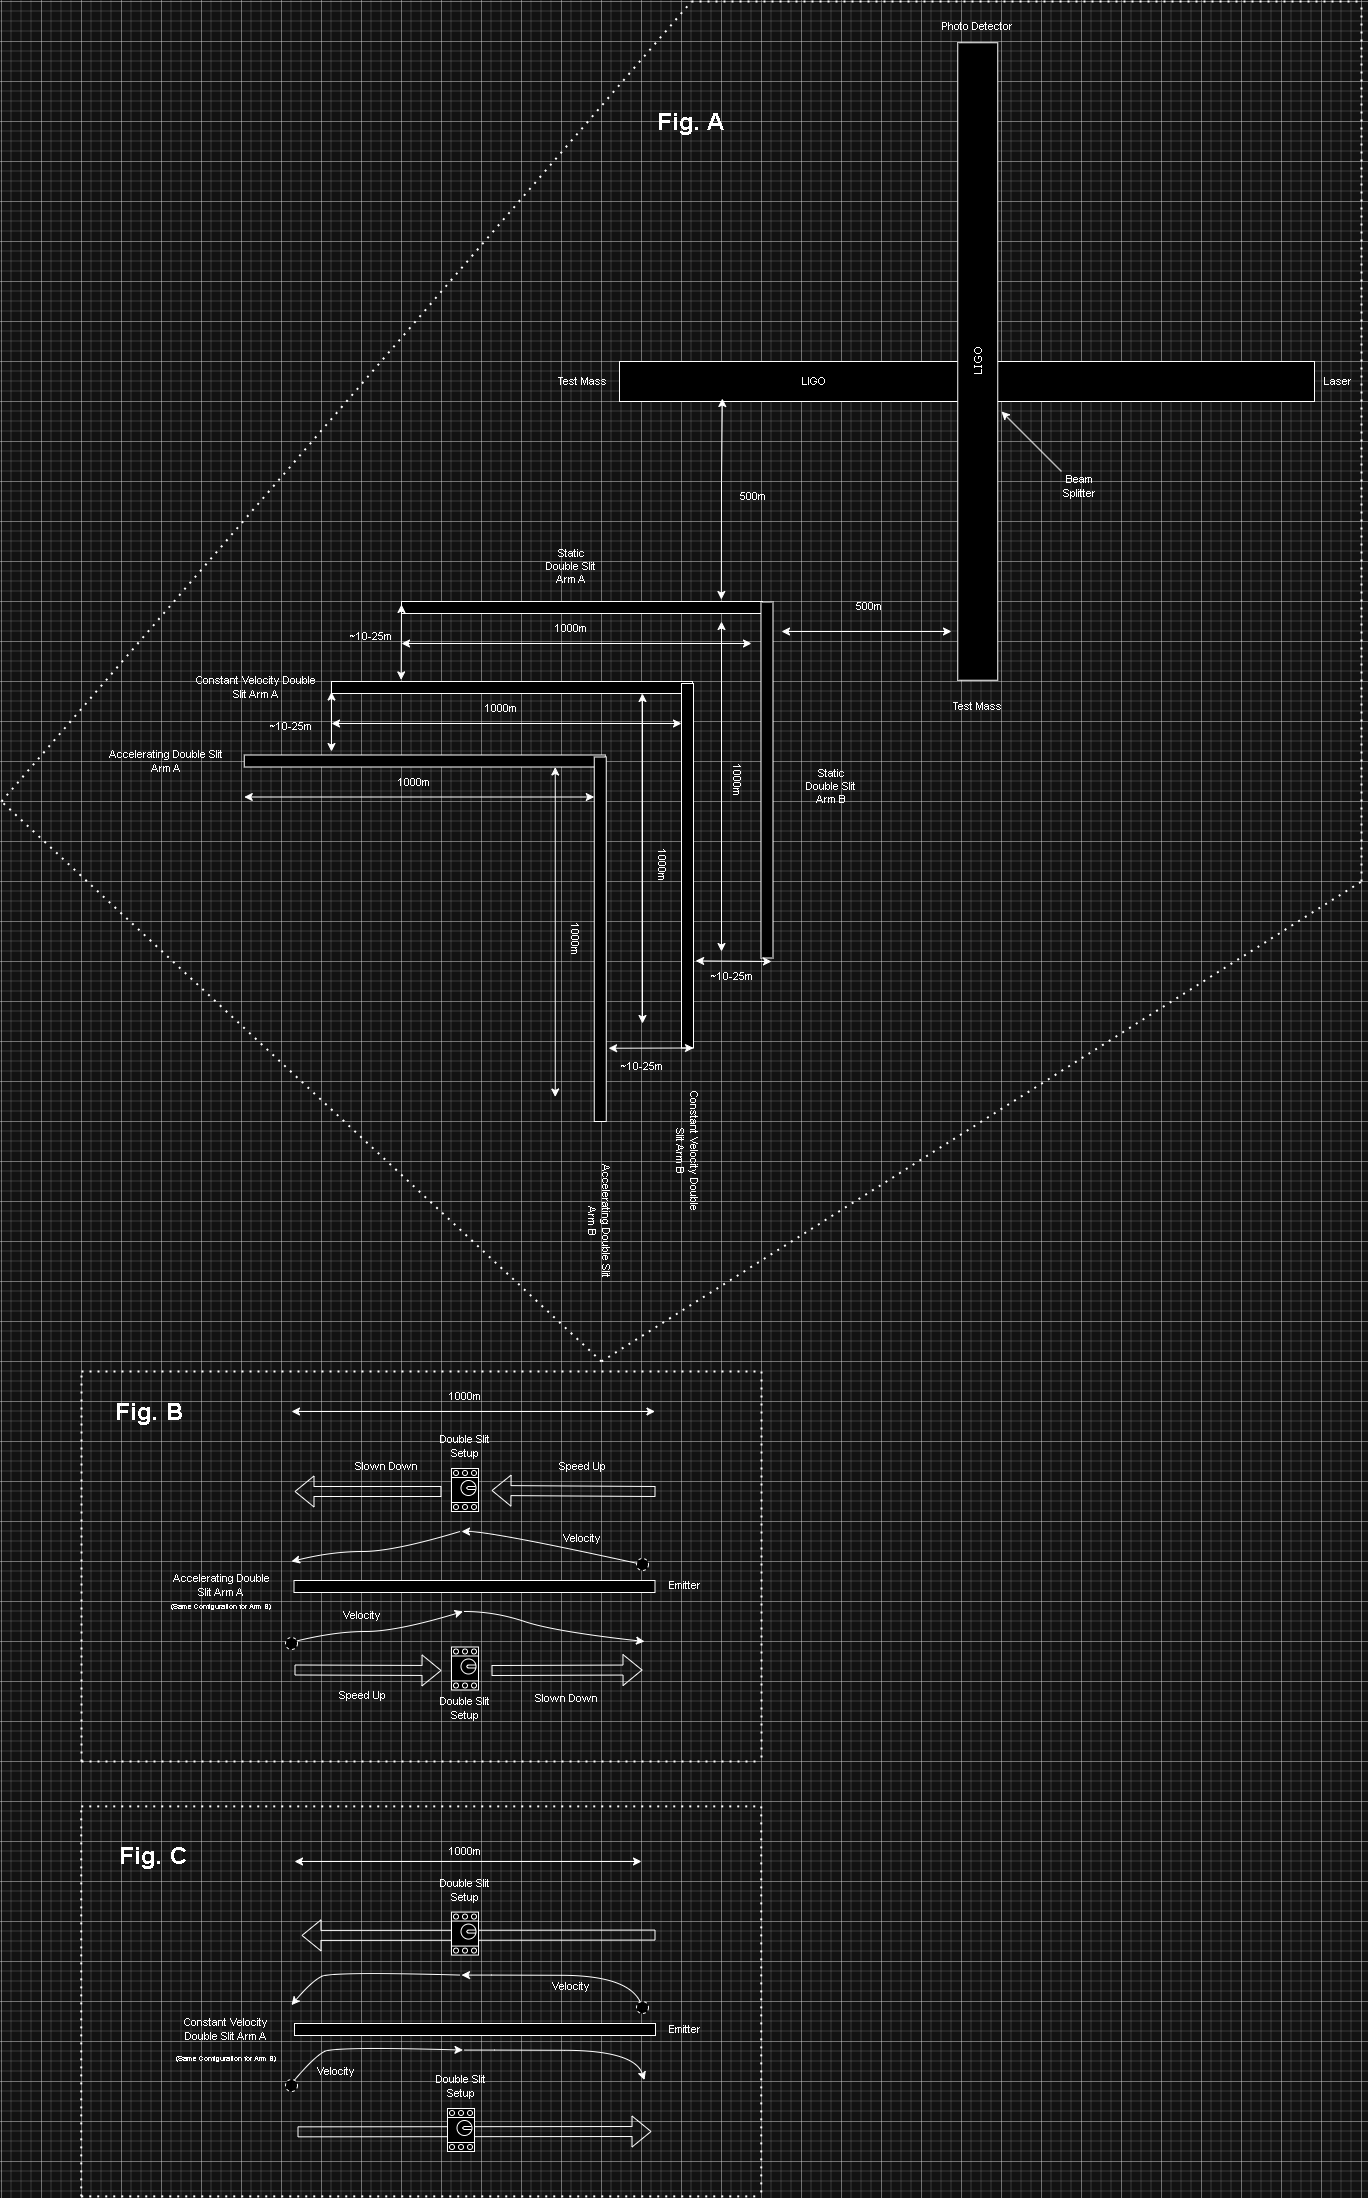
\includegraphics[width=0.60\textwidth]{Schematic-v1.2.2.drawio-dark.png} % Resizes the image to 90% of text width
    \caption{Schematic of the Experimental Setup. This diagram illustrates the experimental configuration used to test the interaction of light with varying velocities in a modified double-slit experiment.}
    \label{fig:experiment_setup}
\end{figure}
\subsection{Overview of the Experimental Setup (Fig. A)}

The primary apparatus consists of the \textbf{LIGO interferometer}, depicted with \textbf{500-meter arms}. A laser source is split by a beam splitter, sending light through the interferometer arms to interact with test masses at each end. Additionally, two \textbf{Double Slit Arms (A and B)} are positioned to analyze how light behaves when it passes through slits at varying velocities (accelerating and constant velocities). The light beams from these arms are designed to interact with the test masses in the interferometer, measuring any resulting interference patterns.

\textbf{Explanation:} This setup uses LIGO's precision to measure potential fluctuations in the interference pattern caused by changes in light speed or acceleration through the double-slit apparatus. The concept draws upon the principles of interferometry, similar to LIGO's gravitational wave detection, but here, the goal is to measure shifts induced by light passing through accelerated or constant-velocity slits.

\subsection{Velocity-Dependent Double Slit Arms (Fig. B and Fig. C)}

\textbf{Fig. B}: Shows the accelerating \textbf{Double Slit Arm A}, where light slows down and speeds up as it passes through the arm.
\begin{itemize}
    \item \textbf{Key Observation:} The relationship between velocity and interference is studied by monitoring how variations in light speed (from acceleration) affect the diffraction pattern. As the light slows and speeds up, it interferes with the other static arm.
\end{itemize}

\textbf{Fig. C}: Depicts the constant velocity \textbf{Double Slit Arm B}, where light passes at a uniform speed.
\begin{itemize}
    \item \textbf{Key Observation:} Unlike the accelerating arm, this setup maintains a consistent velocity, allowing for a baseline measurement. Differences between this and the accelerating arm provide insight into how velocity fluctuations affect light’s behavior when passing through slits.
\end{itemize}

\textbf{Explanation:} These figures present two key configurations for studying light behavior under different velocity conditions. \textbf{Figure B} addresses acceleration's effect on light passing through the slits, while \textbf{Figure C} provides a control for constant velocity. The contrast between these results is expected to highlight how varying speeds influence the interference pattern in a measurable way.

\subsection{GitHub Repository Reference}

All schematics and experimental setups are available in the \textbf{GitHub repository} at \url{https://github.com/DavidZalewski/Paper-Investigating-Quantum-Behavior-Under-Gravitational-Waves}. The raw \textbf{draw.io} file can be found in the \textbf{Diagrams} folder within the repository for further inspection and modification.

For those wishing to inspect the schematic in detail or modify it, the \textbf{draw.io} file can be opened with the Draw.io application (available online or as a desktop app). Images of the schematic in \textbf{JPEG/PNG} format are also provided for quick reference.

\section{Discussion}

\subsection{Interpretation of Results}
The anticipated results from this experiment could offer profound insights into the behavior of quantum particles under the influence of gravitational waves. If the interference patterns of electrons show significant variation when subjected to gravitational waves, it would suggest a coupling between quantum mechanics and gravitational effects, hinting at a deeper connection between the two realms of physics.

1. \textbf{Impact of Gravitational Waves on Quantum Behavior}: If the moving double slit experiment demonstrates a measurable change in interference patterns corresponding to detected gravitational waves, this could imply that gravitational waves exert an influence on quantum particles beyond mere space-time curvature. Such results might support the idea that gravity affects quantum systems in a way that is currently not accounted for in existing quantum field theories.

2. \textbf{Role of Motion in Quantum Systems}: The moving double slit setup allows for exploration of how motion affects the wave function of particles. Should the results indicate observable differences in interference patterns based on the velocity of the slits, it may suggest that the dynamics of a system significantly alter the behavior of quantum particles. This would resonate with concepts such as the Doppler effect and how it could extend into quantum domains, challenging the traditional notions of static particle behavior.

3. \textbf{Validation of Quantum Gravity Theories}: If significant correlations are found between the gravitational wave events detected by LIGO and variations in quantum interference patterns, it could lend credence to theoretical frameworks that attempt to unify gravity with quantum mechanics, such as loop quantum gravity or string theory. These frameworks posit that spacetime itself may have a quantized structure, and observing their effects at this level could provide critical empirical support.

\subsection{Limitations}
While the proposed experiment presents an innovative approach to exploring these fundamental questions, certain limitations must be acknowledged:

1. \textbf{Detection Sensitivity}: The ability to detect subtle changes in interference patterns due to gravitational wave interactions is contingent on the sensitivity of the detection apparatus. Existing technology may need refinement to ensure that the experimental setup can discern these effects amidst background noise. 

Another potential challenge arises from the brief duration of gravitational wave observations at LIGO, which may last on the order of nanoseconds or shorter. If the time window of observation is extremely narrow, it becomes critical to synchronize the experiment’s timing mechanisms, such as the slits’ control system, with the detection timestamps provided by LIGO. To achieve this, atomic clocks will be employed to ensure that any changes at the slits are properly correlated with the gravitational wave event. This high level of precision is necessary to mitigate the effects of the minute delay introduced by the finite travel time of the gravitational wave.

2. \textbf{Underlying Assumptions}: The same limitations inherent in the traditional double slit experiment and LIGO's design will apply here. Both systems depend on idealized conditions to observe quantum behavior, and deviations from these conditions could complicate results. Factors such as decoherence, environmental disturbances, and measurement-induced changes must be carefully controlled and accounted for to ensure the validity of the findings.

3. \textbf{Data Collection Methods}: Data collected in this experiment could utilize both analog and digital methods, each with its respective strengths and weaknesses. Analog systems have a long history of reliability and may provide more straightforward measurements in certain contexts. In contrast, digital systems, while beneficial for processing and analyzing data, are susceptible to errors or bugs in algorithms that could lead to erroneous outputs. Therefore, employing both methods may enhance confidence in the results, allowing for cross-validation of findings. Should discrepancies arise between the two data types, favoring analog data may be prudent, given its extensive testing and validation in various applications.

\section{Future Considerations}

Several potential modifications and extensions to the experiment could provide deeper insights into quantum phenomena. These include:

1. \textbf{Different Mediums for the Double Slit}: The experiment could be repeated using various mediums, such as liquid water, hydrogen gas, or strong electromagnetic fields, to observe how the emitter interacts with these environments. 

2. \textbf{Incorporating Aerodynamics}: Introducing aerodynamics into the double slit setup may lead to interesting observations at the quantum level, particularly with respect to how airflow or pressure variations influence particle behavior.

3. \textbf{Moving Emitters}: Modifying the emitter so that it is also in motion during the experiment may yield new insights into quantum phenomena, especially regarding the wave function collapse in dynamic systems.

4. \textbf{Variety of Emitters}: Using different types of emitters, such as photons, neutrons, or protons, could reveal how various force carrier particles behave in a double-slit setup and how their wave function collapse differs from electrons.

5. \textbf{Tunneling Barriers}: Introducing a barrier where quantum tunneling is predicted to occur, and studying the interference patterns when either the barrier or the emitter is in motion, could provide novel insights into tunneling effects.

6. \textbf{Plasma Barriers}: Modifying the double slit to include a plasma barrier (e.g., fire) before the measurement stage could offer an opportunity to study how the interference pattern of particles changes when interacting with a plasma medium.


\printbibliography

\end{document}